The goal of this research is to be able to provide a system that makes use of an Arduino-based measuring device that can pass on data with a Bluetooth module to an Android phone that can be able to relay this data to a firebase database that can be accessed by another Android phone.

In order to be able to verify the temperature-humidity sensor being used, another device will serve as the basis for true data. Measurements coming from the TH-65, a digital temperature and humidity measuring device, will be established as ground truth.

The following graphs show the accuracy testing of the DHT-11 with the TH-65 as the basis for ground truth. The blue data represents the temperature measured by the DHT-11 while the orange represents data coming from the TH-65. Temperature, humidity, and discomfort index are to be considered in this set of data. From the results, it has been shown that in measuring temperature, the DHT-11 sensor shows 98.91\% accuracy and in humidity, the sensor is 89.66\% accurate in terms of measuring humidity and in discomfort index, the sensor is 97.79\% accurate. %The DHT-11 is shown to be 97.79\% accurate regarding the digital thermometer-hygrometer.

\begin{figure}[h]
\centering
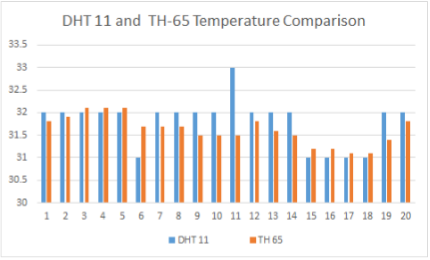
\includegraphics{Temperature}
\caption{Accuracy Testing of Temperature from DHT-11 sensor}
\end{figure}

\begin{figure}[h]
\centering
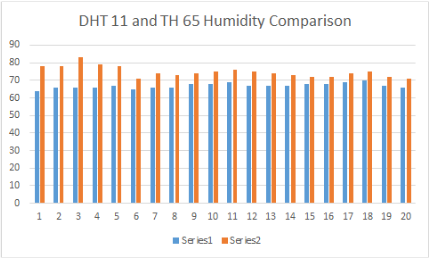
\includegraphics{Humidity}
\caption{Accuracy Testing of Humidity from DHT-11 sensor}
\end{figure}

\begin{figure}[h]
\centering
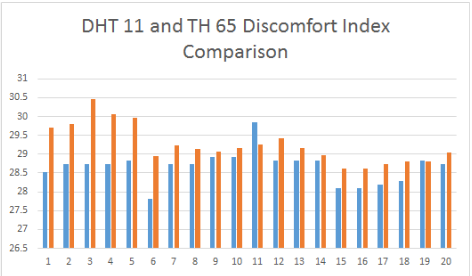
\includegraphics{DI}
\caption{Accuracy Testing of Discomfort Index from DHT-11 sensor}
\end{figure}

\section{Summary}